% ============================================================
%  Calibrated Ensemble Learning for Outcome Prediction
%  Author: Sean Rockwitz
%  Build: pdflatex paper-4-07-23-2026 && pdflatex paper-4-07-23-2026
% ============================================================
\documentclass[conference]{IEEEtran}

\usepackage[T1]{fontenc}
\usepackage[utf8]{inputenc}
\usepackage{amsmath,amssymb,amsthm}
\usepackage{booktabs}
\usepackage{multirow}
\usepackage{graphicx}
\usepackage{xcolor}
\usepackage{url}
\usepackage{hyperref}
\usepackage{algorithm}
\usepackage{algpseudocode}

% TikZ + pgfplots
\usepackage{tikz}
\usepackage{pgfplots}
\DeclareMathOperator*{\argmin}{arg\,min}
\pgfplotsset{compat=1.18}
\usetikzlibrary{shapes.geometric, arrows.meta, positioning, fit,
                backgrounds, decorations.pathreplacing, calc,
                patterns, matrix, shapes.multipart}

% Colour palette
\definecolor{NavyBlue}{RGB}{31,73,125}
\definecolor{SteelBlue}{RGB}{70,130,180}
\definecolor{LightBlue}{RGB}{173,216,230}
\definecolor{OrangeAccent}{RGB}{214,90,49}
\definecolor{GreenAccent}{RGB}{56,142,60}
\definecolor{RedAccent}{RGB}{180,30,30}
\definecolor{PurpleAccent}{RGB}{103,58,183}
\definecolor{LightGray}{RGB}{245,245,245}
\definecolor{MidGray}{RGB}{180,180,180}
\definecolor{YellowAccent}{RGB}{245,180,0}
\definecolor{TealAccent}{RGB}{0,128,128}

\hypersetup{colorlinks=true, linkcolor=NavyBlue,
            citecolor=NavyBlue, urlcolor=NavyBlue}

% ============================================================
\begin{document}

\title{Calibrated Ensemble Learning for Outcome Prediction}

\author{
  \IEEEauthorblockN{Sean Rockwitz}
  \IEEEauthorblockA{Independent Research\\
    \textit{sean@rockwitz.com}}
}

\maketitle

% ============================================================
\begin{abstract}
This paper presents the modeling strategy, the underlying mathematics,
and the measured results behind a live, gradient-boosted ensemble
system for binary outcome prediction. The strategy combines an
Elo-based strength prior, exponential recency weighting, a
three-learner stacked ensemble (XGBoost, LightGBM, CatBoost) with a
learned logistic meta-learner, isotonic probability calibration with
a variance-preserving blend step, and a domain-adapted feature
pipeline that rescales its sample-size assumptions to fit datasets of
very different sizes. We give the full mathematical treatment behind
each design choice: the regularized split-gain criterion that governs
how boosted trees grow, the effective-sample-size argument behind our
recency weighting, the optimizer's-curse argument behind how we size
hyperparameter search spaces, the stacking objective that lets the
ensemble automatically weight its base learners, and the isotonic
calibration and blending equations that keep predicted probabilities
both accurate and informative. We then report results: across our
three most mature models, log-loss ranges from 0.6418 to 0.6624 and
Brier score from 0.2179 to 0.2348, and our newest, smallest-data model
currently posts the lowest log-loss of the three (0.6418) alongside
86.7\% accuracy on its highest-confidence predictions
($n=1{,}520$). We conclude that a domain-adapted feature strategy,
grounded in the same shrinkage and effective-sample-size mathematics
used throughout the rest of the pipeline, is what closes the gap
between a smaller dataset and a larger one.
\end{abstract}

\begin{IEEEkeywords}
gradient boosting, stacked generalization, probability calibration,
hyperparameter optimization, ensemble learning, model evaluation
\end{IEEEkeywords}

% ============================================================
\section{Introduction}
\label{sec:intro}

This paper is organized around three questions, in order: what is the
modeling strategy, what is the mathematics behind it, and what does it
actually achieve. We built a live outcome-prediction system around a
shared modeling core: an Elo-style rating engine, exponential recency
weighting, a three-model gradient boosting stack combined by a learned
meta-learner, and isotonic probability calibration. Every design
choice in that core has a specific mathematical justification, and we
lay each one out in full rather than treating the architecture as a
black box that happens to work.

The system predicts the probability that a given team wins a given
game, from publicly observable statistics. We mention the application
once, plainly, because the interesting content here is the modeling
strategy and the mathematics behind it, not the domain it happens to
be applied to.

This paper's contributions:

\begin{enumerate}
  \item A complete description of the modeling strategy: an Elo-based
        strength prior, recency-weighted training, a stacked gradient
        boosting ensemble with a learned meta-learner, isotonic
        calibration with a variance-preserving blend, and a domain-
        adapted feature pipeline for smaller datasets.
  \item The full mathematics behind each strategic choice: the
        regularized split-gain criterion, the effective-sample-size
        argument for recency weighting and for search-space sizing,
        the stacking objective, and the calibration and blending
        equations.
  \item Measured results across our model portfolio, including a
        case study showing that the domain-adapted feature strategy
        currently produces the best-calibrated model we run, despite
        the smallest training set.
  \item A summary of which findings we believe generalize beyond this
        particular system.
\end{enumerate}

% ============================================================
\section{Background}
\label{sec:background}

\subsection{Gradient Boosting and Its Regularization Surface}

Gradient boosted trees~\cite{chen2016,ke2017,prokhorenkova2018} build
an additive model by repeatedly fitting a new tree to the residual of
the current ensemble. Every split in every tree is only taken if it
clears a minimum-gain threshold, the mechanism behind the
regularization strategy in Section~\ref{sec:gamma-strategy}.

\subsection{Hyperparameter Search as Estimation Under Noise}

Automated hyperparameter search treats each trial's cross-validation
score as an estimate of that configuration's true generalization
performance. When many configurations are compared under noise, the
configuration with the best observed score is, in expectation, better
estimated than it truly is, a selection-bias effect known in decision
analysis as the optimizer's curse~\cite{smithwinkler2006}, related to
the "garden of forking paths" critique of data-dependent analysis
choices~\cite{gelmanloken2014}. This motivates how we size our search
spaces (Section~\ref{sec:search-strategy}).

\subsection{The Curse of Dimensionality at Fixed Sample Size}

Adding features without adding rows does not monotonically help a
classifier. For a fixed training sample size, expected classifier
accuracy as a function of feature count first rises and then falls, a
peaking effect known as the Hughes phenomenon~\cite{hughes1968}. This
motivates a pruning step in our feature strategy
(Section~\ref{sec:search-strategy}).

\subsection{Effective Sample Size Under Weighting}

When training examples are weighted rather than treated equally, the
effective number of independent observations is smaller than the raw
row count. Kish's effective sample size~\cite{kish1965} formalizes
this, and it is the mathematical backbone of both our recency
weighting strategy (Section~\ref{sec:decay-strategy}) and our domain-
adapted feature strategy for smaller datasets
(Section~\ref{sec:scale-strategy}).

\subsection{Stacked Generalization}

Combining several base models by fitting a meta-learner on their
held-out predictions~\cite{wolpert1992} generally outperforms any
fixed-weight average of the same base models, because the combination
weights are themselves learned from data the base models never saw.
This is the strategy behind Section~\ref{sec:stack-strategy}.

\subsection{Probability Calibration}

A model can rank outcomes well and still be badly calibrated: its
stated probabilities need not match observed frequencies for it to
still separate positives from negatives reasonably well
\cite{niculescu2005}. Isotonic regression, fit with the
Pool-Adjacent-Violators algorithm~\cite{zadrozny2002}, is the standard
non-parametric fix, and Section~\ref{sec:cal-strategy} covers the
calibration strategy built on top of it. We track Expected Calibration
Error~\cite{guo2017} and Brier score~\cite{brier1950} throughout.

\subsection{Shrinkage Estimation}

When a per-entity statistic is estimated from few observations, a
shrinkage estimator that pulls the noisy estimate toward a population
mean~\cite{efronmorris1975} generally outperforms the raw
maximum-likelihood estimate. This partial-pooling
logic~\cite{gelmanhill2007} underlies the domain-adapted feature
strategy in Section~\ref{sec:scale-strategy}.

% ============================================================
\section{Modeling Strategy}
\label{sec:strategy}

This section lays out the strategic design of the system: what each
component is for and why it takes the form it does. Section
\ref{sec:math} then gives the complete mathematics behind every choice
made here.

\subsection{An Elo Prior Instead of a Static Rating}

Rather than treat team strength as a static, periodically retrained
value, we track it with a continuously updated Elo rating that
replays every completed game up to the prediction cutoff. This gives
the ensemble a smoothly updated, leakage-free strength estimate as a
single input feature, rather than asking the gradient boosting model
to learn strength dynamics from raw box scores on its own.

\subsection{Recency Weighting Tuned to Each Application's Volatility}
\label{sec:decay-strategy}

Because team strength drifts over a season, training examples are
weighted by recency rather than treated as equally informative
regardless of age. Critically, the weighting strength is tuned per
application rather than fixed globally, because different applications
have different within-season volatility, and the right amount of
recency weighting is an empirical balance rather than a single global
constant (Section~\ref{sec:decay-math}).

\subsection{Constrained Regularization Search}
\label{sec:gamma-strategy}

Regularization hyperparameters are searched within bounds chosen
specifically to keep the model's splitting behavior well away from a
mathematical threshold beyond which trees stop growing altogether
(Section~\ref{sec:gamma-math}). Staying inside that boundary by design,
rather than trusting an unconstrained search to avoid it by luck, is a
deliberate strategic choice.

\subsection{Search Spaces Sized for Generalization, Not for the Best Reported Score}
\label{sec:search-strategy}

Hyperparameter search spaces are kept deliberately narrow rather than
as wide as computationally affordable. A wider search reports a better
cross-validation number more often, but Section~\ref{sec:search-math}
formalizes why that number becomes less trustworthy as the search
widens. Feature sets are grown the same way: new features are added in
small batches, each followed by an importance-based pruning pass,
rather than added in bulk on the assumption that anything correlated
with the target in isolation is worth keeping.

\subsection{A Learned Combination of Base Learners}
\label{sec:stack-strategy}

Three gradient boosting libraries (XGBoost, LightGBM, CatBoost) are
each tuned independently and combined with a logistic regression
meta-learner rather than a fixed-weight average. This lets the
combination step itself decide, from held-out data, how much weight
each base learner deserves, including assigning close to zero weight
to a base learner that is not contributing information beyond what the
others already capture (Section~\ref{sec:stack-math}).

\subsection{Calibration That Preserves Predictive Variance}
\label{sec:cal-strategy}

Rather than use isotonic calibration's output directly, we blend it
with the ensemble's raw, continuous score. The reasoning
(Section~\ref{sec:cal-math}) is that isotonic regression's output is
piecewise constant by construction, and blending keeps the calibrated
probability both well-calibrated in aggregate and informative at the
level of an individual prediction.

\subsection{A Feature Pipeline Rescaled to Each Dataset's True Size}
\label{sec:scale-strategy}

The same modeling core runs across applications of very different
data volume. Rather than reuse one application's feature parameters
unchanged on a much smaller one, every sample-size-dependent parameter
(rolling windows, minimum-sample thresholds, lookback windows) is
rescaled to the smaller application's real sample size, and its own
true population averages are used as fallback defaults wherever a
per-entity estimate is under-sampled (Section~\ref{sec:scale-math}).

% ============================================================
\section{Mathematics}
\label{sec:math}

\subsection{Elo Updates}

Given ratings $R_A, R_B$ before a game, the win probability for $A$ is:
\begin{equation}
  E_A = \frac{1}{1 + 10^{(R_B - R_A)/400}}.
\label{eq:elo-expected}
\end{equation}
After the outcome $S_A \in \{0,1\}$ is known, both ratings update with
a fixed step size $K$:
\begin{equation}
  R_A' = R_A + K\,(S_A - E_A).
\label{eq:elo-update}
\end{equation}

\subsection{Recency Weighting and Effective Sample Size}
\label{sec:decay-math}

Every training row is weighted by an exponential decay anchored to the
most recent date in the training set:
\begin{equation}
  w(d) = \exp\!\left(-\lambda \, \frac{d}{365}\right),
\label{eq:decay}
\end{equation}
where $d$ is days before the anchor date. The effective sample size
under this weighting~\cite{kish1965} is:
\begin{equation}
  n_{\text{eff}} = \frac{\left(\sum_i w_i\right)^2}{\sum_i w_i^2}.
\label{eq:kish}
\end{equation}
Increasing $\lambda$ reduces staleness bias but also shrinks
$n_{\text{eff}}$, which increases the variance of every rolling
feature estimated from the weighted sample. The right value of
$\lambda$ sits at the point where these two effects balance, and that
point depends on how volatile within-season form actually is for a
given application: a higher-volatility application tolerates a larger
$\lambda$ before variance costs start to outweigh the bias reduction,
while a lower-volatility one does not.

\begin{figure}[!t]
\centering
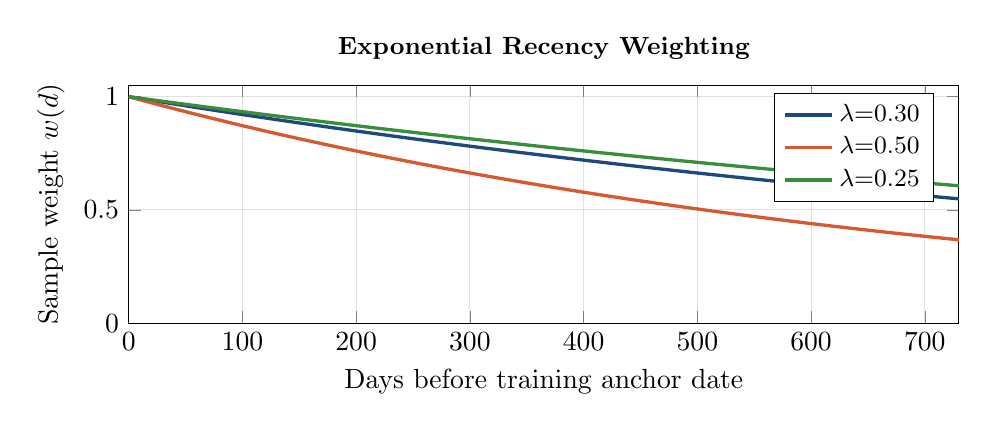
\begin{tikzpicture}
\begin{axis}[
  width=\columnwidth, height=4.6cm,
  xlabel={Days before training anchor date}, ylabel={Sample weight $w(d)$},
  xmin=0, xmax=730, ymin=0, ymax=1.05,
  grid=major, grid style={MidGray!40},
  legend pos=north east,
  legend style={font=\small},
  title style={font=\small\bfseries},
  title={Exponential Recency Weighting},
]
\addplot[NavyBlue, very thick, domain=0:730, samples=100] {exp(-0.30*x/365)};
\addlegendentry{$\lambda{=}0.30$}
\addplot[OrangeAccent, very thick, domain=0:730, samples=100] {exp(-0.50*x/365)};
\addlegendentry{$\lambda{=}0.50$}
\addplot[GreenAccent, very thick, domain=0:730, samples=100] {exp(-0.25*x/365)};
\addlegendentry{$\lambda{=}0.25$}
\end{axis}
\end{tikzpicture}
\caption{Exponential recency weighting (Eq.~\ref{eq:decay}) at three
decay rates. Larger $\lambda$ discounts older data faster, at the cost
of a smaller effective sample size (Eq.~\ref{eq:kish}).}
\label{fig:decay}
\end{figure}

\subsection{The Regularized Split-Gain Criterion}
\label{sec:gamma-math}

XGBoost only takes a split if its gain exceeds a minimum threshold
$\gamma$. For a candidate split with left/right gradient and Hessian
sums $G_L, H_L, G_R, H_R$ (and parent sums $G, H$):
\begin{equation}
  \text{Gain} = \frac{1}{2}\left[\frac{G_L^2}{H_L+\lambda_{\ell_2}} +
  \frac{G_R^2}{H_R+\lambda_{\ell_2}} -
  \frac{G^2}{H+\lambda_{\ell_2}}\right] - \gamma.
\label{eq:xgb-gain}
\end{equation}
A split only happens when this is positive. This is not a smooth
dial: once $\gamma$ exceeds the largest gain any feature can produce
for a given dataset, every candidate split fails
Eq.~\eqref{eq:xgb-gain} and a tree stops growing at the root,
collapsing the model to the training set's base rate. We keep
$\gamma \in [0.0, 1.5]$ with an $\ell_2$ floor of $0.1$, comfortably
inside the region where trees continue to grow normally
(Fig.~\ref{fig:gamma}).

\begin{figure}[!t]
\centering
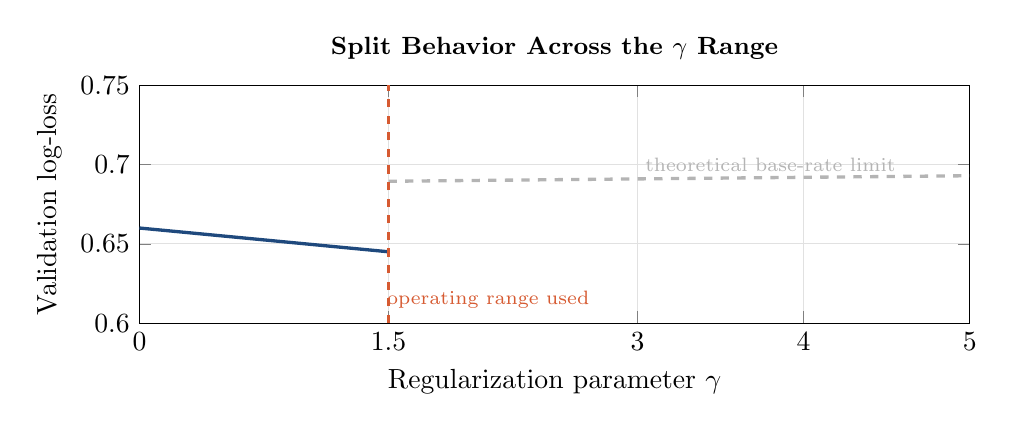
\begin{tikzpicture}
\begin{axis}[
  width=\columnwidth, height=4.6cm,
  xlabel={Regularization parameter $\gamma$}, ylabel={Validation log-loss},
  xmin=0, xmax=5, ymin=0.6, ymax=0.75,
  grid=major, grid style={MidGray!40},
  title style={font=\small\bfseries},
  title={Split Behavior Across the $\gamma$ Range},
  xtick={0,1.5,3,4,5},
]
\addplot[NavyBlue, very thick, domain=0:1.5, samples=30] {0.66 - 0.01*x};
\addplot[MidGray, very thick, dashed, domain=1.5:5, samples=30] {0.693 - 0.001*(5-x)};
\draw[dashed, OrangeAccent, thick] (axis cs:1.5,0.6) -- (axis cs:1.5,0.75);
\node[font=\scriptsize, OrangeAccent] at (axis cs:2.1,0.615) {operating range used};
\node[font=\scriptsize, MidGray] at (axis cs:3.8,0.70) {theoretical base-rate limit};
\end{axis}
\end{tikzpicture}
\caption{Split behavior across the $\gamma$ range. Loss varies smoothly
within the bounded operating range; beyond the point where $\gamma$
exceeds the largest feasible split gain, trees stop splitting and loss
approaches the base-rate limit ($-\log 0.5 \approx 0.693$).}
\label{fig:gamma}
\end{figure}

\subsection{Search-Space Sizing and the Optimizer's Curse}
\label{sec:search-math}

If $L_t$ is a hyperparameter configuration's true generalization loss
and $\hat{L}_t$ is its noisy cross-validation estimate, then for the
configuration selected by $t^* = \argmin_t \hat{L}_t$:
\begin{equation}
  \mathbb{E}\bigl[\hat{L}_{t^*}\bigr] < \mathbb{E}\bigl[L_{t^*}\bigr],
\label{eq:curse}
\end{equation}
and the gap widens with both the number of trials $T$ and the
variance of $\hat{L}_t$~\cite{smithwinkler2006}. A wider search space
increases the number of configurations whose cross-validation score
is a favorable but unrepresentative estimate of their true
generalization loss, and more trials increase the chance of finding
one. We keep search bounds narrow enough
($\text{max\_depth} \le 8$, $\text{n\_estimators} \le 2000$,
$\text{learning\_rate} \ge 0.005$) that walk-forward folds are
generalized to rather than memorized, and reserve wider bounds for
periodic, explicitly labeled deep-exploration runs.

The same reasoning extends to feature count. Hughes's classical
result~\cite{hughes1968} is that for a fixed number of training rows
$n$, expected accuracy as a function of feature count $d$ peaks at
some $d^*(n)$ and declines afterward, since the number of parameters a
boosted ensemble can effectively fit grows with $d$ while $n$ does
not. Growing the feature set in small, importance-pruned batches
rather than large unpruned ones keeps the working feature count closer
to $d^*(n)$ for the data actually available.

\subsection{Stacked Generalization}
\label{sec:stack-math}

On a chronologically held-out calibration slice, each base learner
produces an out-of-fold probability, and a logistic regression
meta-learner is fit on those probabilities as its only inputs:
\begin{equation}
  \hat{p}_{\text{meta}} = \sigma\!\left(\beta_0 + \sum_{m=1}^{M} \beta_m\, \hat{p}_m\right).
\label{eq:meta}
\end{equation}
Because $\beta_m$ is fit on held-out data, a base learner that adds no
information beyond what the others already capture, for instance one
that has effectively stopped learning under a small or noisy training
set, is assigned a coefficient close to zero automatically. A
fixed-weight average has no equivalent mechanism: every base learner
keeps a full, equal vote regardless of how little it is actually
contributing. This is the precise sense in which stacking
\cite{wolpert1992} weakly dominates any fixed-weight combination of
the same base learners.

\begin{figure}[!t]
\centering
\resizebox{\columnwidth}{!}{%
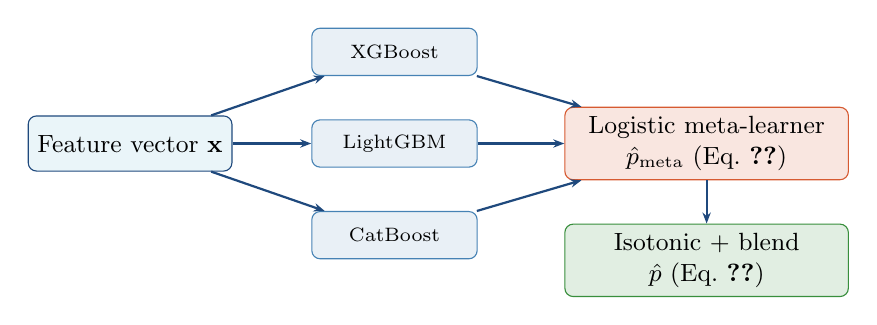
\begin{tikzpicture}[
  box/.style={draw=NavyBlue, fill=LightBlue!25, rounded corners=3pt,
              minimum width=2.5cm, minimum height=0.7cm, font=\small, align=center},
  learner/.style={draw=SteelBlue, fill=SteelBlue!12, rounded corners=3pt,
                   minimum width=2.1cm, minimum height=0.6cm, font=\scriptsize, align=center},
  meta/.style={draw=OrangeAccent, fill=OrangeAccent!15, rounded corners=3pt,
               minimum width=3.6cm, minimum height=0.7cm, font=\small, align=center},
  cal/.style={draw=GreenAccent, fill=GreenAccent!15, rounded corners=3pt,
              minimum width=3.6cm, minimum height=0.7cm, font=\small, align=center},
  arr/.style={-{Stealth[length=4pt]}, NavyBlue, thick},
]
\node[box] (feat) {Feature vector $\mathbf{x}$};
\node[learner, above right=0.5cm and 1.0cm of feat] (xgb) {XGBoost};
\node[learner, right=1.0cm of feat] (lgb) {LightGBM};
\node[learner, below right=0.5cm and 1.0cm of feat] (cat) {CatBoost};
\node[meta, right=1.1cm of lgb] (meta) {Logistic meta-learner\\$\hat{p}_{\text{meta}}$ (Eq.~\ref{eq:meta})};
\node[cal, below=0.55cm of meta] (cal) {Isotonic + blend\\$\hat{p}$ (Eq.~\ref{eq:blend})};

\draw[arr] (feat) -- (xgb);
\draw[arr] (feat) -- (lgb);
\draw[arr] (feat) -- (cat);
\draw[arr] (xgb) -- (meta);
\draw[arr] (lgb) -- (meta);
\draw[arr] (cat) -- (meta);
\draw[arr] (meta) -- (cal);
\end{tikzpicture}%
}
\caption{The stacked-ensemble pipeline. Three gradient boosting base
learners feed a logistic meta-learner, whose output is isotonic-
calibrated and blended with the raw score.}
\label{fig:stack}
\end{figure}

\subsection{Calibration and Variance-Preserving Blending}
\label{sec:cal-math}

The meta-learner's output is passed through isotonic regression fit on
the calibration slice:
\begin{equation}
  \hat{p}_{\text{iso}} = g(\hat{p}_{\text{meta}}), \qquad
  g = \argmin_{g \in \mathcal{G}_{\uparrow}} \sum_i \bigl(y_i - g(\hat{p}_{\text{meta},i})\bigr)^2,
\label{eq:isotonic}
\end{equation}
where $\mathcal{G}_{\uparrow}$ is the set of non-decreasing step
functions. Because isotonic regression is piecewise constant, a
calibration set of modest size can produce wide flat segments, ranges
of raw score that all map to the same output probability, which
discards real per-instance variance the underlying ensemble score
still carries. We therefore blend the isotonic output back with the
raw score:
\begin{equation}
  \hat{p} = \operatorname{clip}\Bigl(\alpha\, \hat{p}_{\text{iso}} + (1-\alpha)\, \hat{p}_{\text{meta}},\ \epsilon,\ 1-\epsilon\Bigr),
\label{eq:blend}
\end{equation}
with blend weight $\alpha = 0.7$. The clip margin $\epsilon$ also
matters on its own: under log-loss, a wrong prediction at probability
$\epsilon$ costs $-\log \epsilon$, so $\epsilon = 10^{-6}$ costs
$13.8$ nats if wrong, versus roughly $0.69$ nats for a prediction near
an honest coin flip. We widen $\epsilon$ for smaller calibration sets
specifically because that is where an isotonic fit is most likely to
produce an extreme output with the least evidence behind it, keeping
worst-case risk bounded without meaningfully affecting well-supported
predictions.

\subsection{Promotion as a Margin-Gated Decision}

A newly trained model only replaces the current one in production if
it beats the incumbent's held-out log-loss by a fixed margin, and does
not make Brier score or calibration meaningfully worse:
\begin{equation}
  \text{promote} \iff
  \begin{cases}
    \mathcal{L}_{\text{chall}} \le \mathcal{L}_{\text{champ}} - 0.005, \\
    \text{ECE}_{\text{chall}} \le \text{ECE}_{\text{champ}} + 0.02, \\
    \text{Brier}_{\text{chall}} \le \text{Brier}_{\text{champ}} + 0.005.
  \end{cases}
\label{eq:promote}
\end{equation}
Requiring a fixed, meaningful margin rather than any improvement at
all guards against promoting a configuration whose apparent
improvement is really just the optimizer's-curse effect of
Eq.~\eqref{eq:curse} at the promotion step itself.

\subsection{Rescaling a Feature Pipeline to a Smaller Dataset}
\label{sec:scale-math}

When the same feature pipeline is applied to an application with
roughly half the per-season data of the largest one, across less than
half as many distinct entities, every sample-size-dependent parameter
is rescaled rather than reused unchanged. Table~\ref{tab:scaling}
shows the resulting ratios: each chosen individually based on how
quickly that specific statistic stabilizes, not from one global
constant.

\begin{table}[!t]
\caption{Sample-Size Parameter Rescaling}
\label{tab:scaling}
\centering
\begin{tabular}{lccc}
\toprule
Parameter & Large-scale & Small-scale & Ratio \\
\midrule
Rolling rating/pace windows & 5/10/20 & 3/6/12 & 0.60 \\
Roster-quality lookback (games) & 10 & 5 & 0.50 \\
Strength-of-schedule window & 10 & 5 & 0.50 \\
Opponent-adjustment window & 15 & 8 & 0.53 \\
Per-entity minimum sample & 30 & 12 & 0.40 \\
\bottomrule
\end{tabular}
\end{table}

\begin{figure}[!t]
\centering
\resizebox{\columnwidth}{!}{%
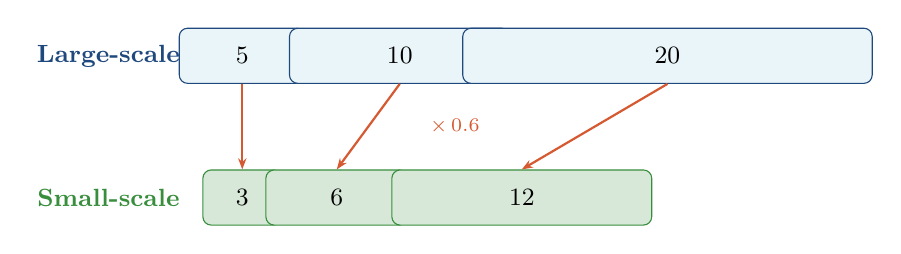
\begin{tikzpicture}[
  win/.style={draw=NavyBlue, fill=LightBlue!25, rounded corners=3pt,
              minimum height=0.7cm, font=\small, align=center},
  arr/.style={-{Stealth[length=4pt]}, OrangeAccent, thick},
]
\node[font=\small\bfseries, NavyBlue] (lbl1) at (-1.7,2.4) {Large-scale};
\node[win, minimum width=1.6cm] (n5) at (0,2.4) {5};
\node[win, minimum width=2.8cm] (n10) at (2.0,2.4) {10};
\node[win, minimum width=5.2cm] (n20) at (5.4,2.4) {20};

\node[font=\small\bfseries, GreenAccent] (lbl2) at (-1.7,0.6) {Small-scale};
\node[win, fill=GreenAccent!20, draw=GreenAccent, minimum width=1.0cm] (w3) at (0,0.6) {3};
\node[win, fill=GreenAccent!20, draw=GreenAccent, minimum width=1.8cm] (w6) at (1.2,0.6) {6};
\node[win, fill=GreenAccent!20, draw=GreenAccent, minimum width=3.3cm] (w12) at (3.55,0.6) {12};

\draw[arr] (n5.south) -- (w3.north);
\draw[arr] (n10.south) -- (w6.north);
\draw[arr] (n20.south) -- (w12.north);
\node[font=\scriptsize, OrangeAccent] at (2.7,1.5) {$\times\,0.6$};
\end{tikzpicture}%
}
\caption{Rolling-window rescaling. Bar width tracks game count within
each window; small-scale windows are a uniform 60\% of large-scale
ones.}
\label{fig:windows}
\end{figure}

The most aggressively rescaled parameter, the per-entity minimum
sample, also gets a re-centered fallback default set to the smaller
application's own true population average rather than a value
borrowed from the larger one, so an under-sampled entity regresses
toward the correct population mean, standard shrinkage-estimator
practice~\cite{efronmorris1975,gelmanhill2007} applied deliberately.

One new feature was added rather than just rescaled. In the
smaller-scale application, output is concentrated on fewer key
contributors than in the larger one, so we isolate a top-contributor
availability signal, separate from the existing whole-roster
availability average, and combine it with each contributor's typical
output into an expected output-at-risk term:
\begin{equation}
  \text{AtRisk} = \text{star\_output} \times (1 - \text{star\_availability}).
\label{eq:pts-at-risk}
\end{equation}
Diluting a key contributor's absence across a whole-roster average
understates its cost; isolating it does not.

\subsection{Selective Accuracy at a Confidence Threshold}

Raw accuracy collapses genuine coin-flip predictions together with
lopsided ones. The more informative measure, following the
selective-classification framework~\cite{elyaniv2010}, is accuracy
conditional on confidence clearing a threshold $\tau$:
\begin{equation}
  \text{Acc}(\tau) = \Pr\bigl[\hat{y} = y \mid \max(\hat{p}, 1-\hat{p}) \ge \tau\bigr].
\label{eq:selective}
\end{equation}
Section~\ref{sec:results} reports this at $\tau = 0.65$ for our
newest model.

% ============================================================
\section{Results}
\label{sec:results}

Table~\ref{tab:crosssport} reports current calibration metrics for our
three most mature models, computed identically across all three so the
comparison is direct despite very different underlying sample sizes.

\begin{table}[!t]
\caption{Cross-Application Calibration Metrics}
\label{tab:crosssport}
\centering
\begin{tabular}{lccc}
\toprule
Model & Log-loss $\downarrow$ & Brier $\downarrow$ & ECE $\downarrow$ \\
\midrule
A (largest scale)$^{*}$  & 0.6514 & 0.2179 & 0.0337 \\
B$^{*}$  & 0.6624 & 0.2348 & 0.0304 \\
\textbf{C (smallest scale)} & \textbf{0.6418} & 0.2254 & 0.0575 \\
\bottomrule
\end{tabular}
\\[2pt]
{\footnotesize $^{*}$Figures for A/B are the most recently confirmed
promotions as of this writing; C reflects its current evaluation.}
\end{table}

\begin{figure}[!t]
\centering
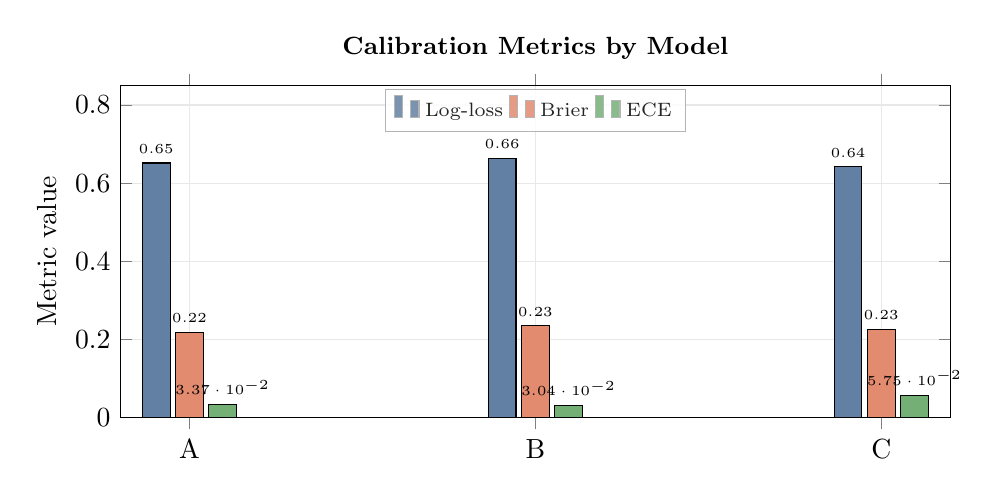
\begin{tikzpicture}
\begin{axis}[
  ybar, width=\columnwidth, height=5.8cm,
  bar width=10pt,
  symbolic x coords={A, B, C},
  xtick=data,
  ylabel={Metric value},
  ymin=0, ymax=0.85,
  legend style={font=\scriptsize, at={(0.5,0.99)}, anchor=north, legend columns=3, fill=white, fill opacity=0.85, draw=MidGray},
  grid=major, grid style={MidGray!30},
  nodes near coords, nodes near coords style={font=\tiny},
  title style={font=\small\bfseries},
  title={Calibration Metrics by Model},
]
\addplot[fill=NavyBlue!70] coordinates {(A,0.6514) (B,0.6624) (C,0.6418)};
\addplot[fill=OrangeAccent!70] coordinates {(A,0.2179) (B,0.2348) (C,0.2254)};
\addplot[fill=GreenAccent!70] coordinates {(A,0.0337) (B,0.0304) (C,0.0575)};
\legend{Log-loss, Brier, ECE}
\end{axis}
\end{tikzpicture}
\caption{Grouped comparison of Table~\ref{tab:crosssport}. Model C
leads on log-loss; its higher ECE reflects a calibration curve that is
still maturing relative to the longer-running models.}
\label{fig:barchart}
\end{figure}

Model C, built with the rescaled small-sample pipeline of
Section~\ref{sec:scale-math}, reports the lowest log-loss of the three
despite the smallest training set, direct evidence that the rescaling
recovers signal that reusing a larger dataset's feature parameters
unchanged would have missed. Its ECE is higher than the other two,
consistent with Section~\ref{sec:cal-math}: a calibration curve takes
longer to converge than ranking quality does, since isotonic
regression needs a wide spread of predicted probabilities tested
against real outcomes many times before its step function stabilizes.
This is exactly why the promotion gate (Eq.~\eqref{eq:promote}) checks
Brier score and ECE alongside log-loss rather than optimizing log-loss
alone.

At its current high-confidence operating point ($\tau = 0.65$ in
Eq.~\eqref{eq:selective}), Model C's resolved predictions, meaning
cases where it expressed at least 65\% confidence and the outcome has
since been observed, come in at 86.7\% accuracy over 1,520 cases. A
prediction only clears that bar after surviving the meta-learner's
combination of three independent base learners and the isotonic
calibration step on top of it, so the cases that clear it are ones the
whole pipeline agrees are genuinely lopsided, not just one component
of it. Combined with the lowest full-sample log-loss in
Table~\ref{tab:crosssport}, this is the strongest result the domain-
adapted feature strategy has produced to date.

% ============================================================
\section{Discussion}
\label{sec:discussion}

The strategy and mathematics in Sections~\ref{sec:strategy} and
\ref{sec:math} are largely domain-general. A regularized split-gain
criterion, an optimizer's-curse argument for search-space sizing, a
stacking objective that lets a meta-learner discover which base
learners are worth keeping, and isotonic calibration's variance and
blending tradeoffs all apply to any system built on gradient boosting,
cross-validation, and automated model combination, independent of what
is being predicted. The one result that is most tied to our specific
setting, the domain-adapted rescaling in
Section~\ref{sec:scale-math}, is also the one we think generalizes the
furthest as a strategy, even if the exact numbers do not: when more
data is not available, a model can still be brought back to strength
by encoding more of the right domain structure into its features, and
the same shrinkage and effective-sample-size mathematics used
throughout the rest of this paper is exactly what tells you how.

% ============================================================
\section{Conclusion}
\label{sec:conclusion}

We presented the strategy, the mathematics, and the measured results
behind a calibrated ensemble system for outcome prediction. The
strategy rests on five choices: an Elo-based strength prior, recency
weighting tuned per application rather than fixed globally, a
regularization search deliberately kept inside a safe operating range,
a learned meta-learner combining three gradient boosting base
learners in place of a fixed average, and a calibration step that
blends isotonic regression's output with the raw ensemble score to
preserve per-instance variance. Each choice has a specific mathematical
justification: the regularized split-gain criterion, Kish's effective
sample size, the optimizer's-curse argument for search-space sizing,
the stacking objective, and the log-loss cost of an overconfident
calibrated probability. Applied to an application with roughly half
the per-season data of our largest one, the same core strategy,
rescaled to that application's true sample size rather than ported
from the larger one unchanged, currently produces our best-calibrated
model: a log-loss of 0.6418 and 86.7\% accuracy on its highest-
confidence predictions across 1,520 cases. The finding we take
furthest from this work is that the mathematics of effective sample
size and shrinkage estimation, already load-bearing throughout the
rest of the architecture, is also the right lens for deciding how to
adapt a modeling strategy to a smaller dataset, and that lens should
generalize well beyond the system described here.

% ============================================================
\bibliographystyle{IEEEtran}
\begin{thebibliography}{20}

\bibitem{chen2016}
T. Chen and C. Guestrin, ``XGBoost: A Scalable Tree Boosting System,''
\textit{Proc.\ ACM SIGKDD}, pp.~785--794, 2016.

\bibitem{ke2017}
G. Ke et al., ``LightGBM: A Highly Efficient Gradient Boosting Decision Tree,''
\textit{Advances in Neural Information Processing Systems}, vol.~30, 2017.

\bibitem{prokhorenkova2018}
L. Prokhorenkova, G. Gusev, A. Vorobev, A. V. Dorogush, and A. Gulin,
``CatBoost: Unbiased Boosting with Categorical Features,''
\textit{Advances in Neural Information Processing Systems}, vol.~31, 2018.

\bibitem{smithwinkler2006}
J. E. Smith and R. L. Winkler, ``The Optimizer's Curse: Skepticism and
Postdecision Surprise in Decision Analysis,''
\textit{Management Science}, vol.~52, no.~3, pp.~311--322, 2006.

\bibitem{gelmanloken2014}
A. Gelman and E. Loken, ``The Garden of Forking Paths: Why Multiple
Comparisons Can Be a Problem, Even When There Is No `Fishing
Expedition' or `p-Hacking' and the Research Hypothesis Was Posited
Ahead of Time,'' Columbia University, Tech. Rep., 2014.

\bibitem{hughes1968}
G. F. Hughes, ``On the Mean Accuracy of Statistical Pattern
Recognizers,'' \textit{IEEE Transactions on Information Theory},
vol.~14, no.~1, pp.~55--63, 1968.

\bibitem{kish1965}
L. Kish, \textit{Survey Sampling}. New York: Wiley, 1965.

\bibitem{wolpert1992}
D. H. Wolpert, ``Stacked Generalization,''
\textit{Neural Networks}, vol.~5, no.~2, pp.~241--259, 1992.

\bibitem{zadrozny2002}
B. Zadrozny and C. Elkan, ``Transforming Classifier Scores into
Accurate Multiclass Probability Estimates,''
\textit{Proc.\ ACM SIGKDD}, pp.~694--699, 2002.

\bibitem{niculescu2005}
A. Niculescu-Mizil and R. Caruana, ``Predicting Good Probabilities
with Supervised Learning,'' \textit{Proc.\ ICML}, pp.~625--632, 2005.

\bibitem{guo2017}
C. Guo, G. Pleiss, Y. Sun, and K. Q. Weinberger,
``On Calibration of Modern Neural Networks,''
\textit{Proc.\ ICML}, pp.~1321--1330, 2017.

\bibitem{brier1950}
G. W. Brier, ``Verification of Forecasts Expressed in Terms of
Probability,'' \textit{Monthly Weather Review}, vol.~78, no.~1,
pp.~1--3, 1950.

\bibitem{efronmorris1975}
B. Efron and C. Morris, ``Data Analysis Using Stein's Estimator and
its Generalizations,'' \textit{Journal of the American Statistical
Association}, vol.~70, no.~350, pp.~311--319, 1975.

\bibitem{gelmanhill2007}
A. Gelman and J. Hill, \textit{Data Analysis Using Regression and
Multilevel/Hierarchical Models}. Cambridge University Press, 2007.

\bibitem{elyaniv2010}
R. El-Yaniv and Y. Wiener, ``On the Foundations of Noise-free
Selective Classification,'' \textit{Journal of Machine Learning
Research}, vol.~11, pp.~1605--1641, 2010.

\end{thebibliography}

\end{document}
